\documentclass[./main.tex]{subfiles}

\begin{document}
\section{Models}
The following section covers the theory behind the various models that will be introduced in Section \ref{sec:experiments}.

\subsection{Mask R-CNN}
\begin{figure}[htbp]
    \centering
    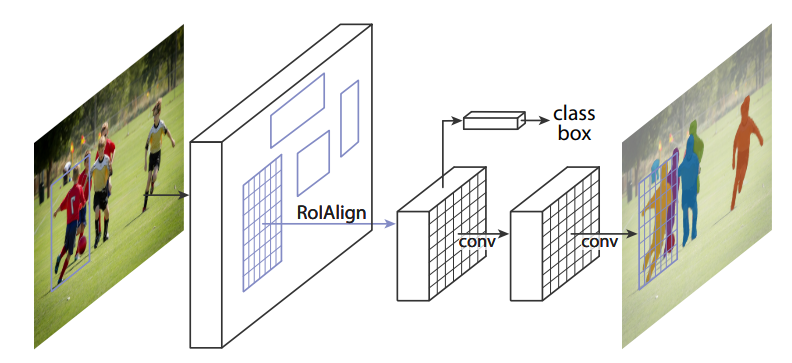
\includegraphics[height=5cm]{./entities/mask_rcnn.PNG}
    \caption{The Mask R-CNN framework for instance segmentation \cite{https://doi.org/10.48550/arxiv.1703.06870}.}
    \label{fig:mask_rcnn}
\end{figure}
\textbf{NOTE: MANGLER NOK AT SKRIVE NOGET MED, AT INPUT ER ET BILLEDE OG LIGNENDE NOGET OM HVAD OUTPUT ER.} \\
\noindent When we will be performing the pose estimation in Section \ref{sec:experiments}, our developed methods will be a variation of the \textit{Mask R-CNN}, introduced by He \textit{et al.} in 2018 \cite{https://doi.org/10.48550/arxiv.1703.06870}. The following subsection explains the architecture of the Mask R-CNN and is based on an interpretation of He \textit{et al.} \cite{https://doi.org/10.48550/arxiv.1703.06870} and Zhang \cite{mask_rcnn_explained}.
\\
\\
The Mask R-CNN can generally be split into various components, which we will explain in further details in the following subsections.

\subsubsection{The Backbone}
The first major component of the Mask R-CNN is the \textit{Backbone}, which is a network used for extracting the features of the input image. Commonly, a pretrained variation of the \textit{residual network} (\textit{ResNet}) is used \cite{https://doi.org/10.48550/arxiv.1512.03385}. The backbone takes an image as input and returns a feature map.

\subsubsection{Region Proposal Network (RPN)}
The next major component of the Mask R-CNN is the \textit{Region Proposal Network} (\textit{RPN}). The RPN takes the feature map from the backbone as input, processes the feature map and proposes regions that may contain an object (the so-called \textit{Region of Interests} or \textit{RoI}) in the form of a feature map. 
\\
\\
The RPN works by first processing the feature map with a convolutional layer that outputs a tensor with $c$ channels, where each spacial vector (also with $c$ channels) is associated with an anchor center. For each of these anchor centers a set of anchor boxes are generated. This convolutional layer is then followed by two $1 \times 1$ convolutional layers that independently processes this tensor. One of these $1 \times 1$ convolutional layers is a binary classifier that predicts whether each anchor box has an object. This is done by mapping each $c$-channel vector to a $k$-channel vector. The other $1 \times 1$ convolutional layer is an object bounding-box regressor, which predicts the offsets between the true object bounding-box and the anchor box. This is done by makking each $c$-channel vector to a $4k$-channel vector. For the overlapping bounding-boxes of the same object, we keep the one with the highest objectness score and discard the rest.

\subsubsection{Region of Interest Alignment (RoIAlign)}
The third major components of the Mask R-CNN is the \textit{Region of Interest Alignment} (\textit{RoIAlign}). This components takes the proposed RoIs from the previous components as input and finds where each RoI is in the feature map. This is done by extracting feature vectors from the output feature map from the RPN and transform them into a fix-sized tensor.

\subsubsection{Object Detection Branch}
\subsubsection{Mask Generation Branch}


\subsection{UniPose-LSTM}

\subsection{DeciWatch}

\end{document}